\documentclass{article}

\PassOptionsToPackage{numbers,sort&compress}{natbib}
% NEmo requires anonymous workshop review. Add `final` only after acceptance.
\usepackage[dblblindworkshop]{neurips_2026}
\workshoptitle{NEmo: Neuro-Symbolic Embodied Intelligence}

\usepackage[utf8]{inputenc}
\usepackage[T1]{fontenc}
\usepackage{courier} % Embedded Type 1 monospace font, including URLs.
\usepackage{amsmath,amssymb}
\usepackage{graphicx}
\usepackage{booktabs}
\usepackage{microtype}
\usepackage{xcolor}
\usepackage[hidelinks]{hyperref}
\usepackage{url}
\graphicspath{{figures/}}
\hypersetup{pdfauthor={},pdftitle={Iterative Policy Refinement through Semantic Rollout Analysis}}

\title{Iterative Policy Refinement through Semantic Rollout Analysis}
\author{Anonymous Author(s)}

\begin{document}
\maketitle

\begin{abstract}
% Structured policies encode task knowledge in a semantically meaningful latent space, providing an inductive bias for efficient learning from demonstrations.
% However, previous work relies on humans to generate the domain knowledge for the task, and prior knowledge of a large language model (LLM) can yield a policy topology that misaligns with the relationships underlying a demonstration.
% We introduce iterative policy structure refinement through semantic rollout analysis.
% Just as a coding agent writes tests to investigate a program's behavior, our method generates tabular data-analysis code from a policy's structure and records its semantic latents during execution.
% The generated code analyzes complete rollout tables and guides structural edits, alternating with parameter fitting on the same demonstration.
% With one demonstration per task, refinement improves Car Racing imitation-learning return by approximately 15\% and reduces the environment resets needed for subsequent reinforcement learning to about 20\% for a similar mean return.
% We also show that it can be generalized to cross other manipulation domains.

Structured policies improve efficiency, robustness, and interpretability in imitation learning by introducing task-specific inductive bias, but existing structure generation methods rely either on extensive human input or on static domain knowledge encoded in LLMs, which may be inconsistent with the expert demonstrations.
We propose a closed-loop framework that iteratively refines structured policies using LLM-guided analysis of policy rollouts.
By logging rollouts as semantically meaningful tabular data and prompting the LLM to generate diagnostic analysis code, our method identifies suboptimalities in the policy structure and iteratively corrects them without requiring human instruction.
Experiments on car racing and door opening tasks show that our approach improves imitation learning performance by up to 15\% over zero-shot LLM-generated structures and requires 75\% less compute to achieve the same reinforcement learning performance.
These results demonstrate that tabular rollout analysis provides an effective feedback signal to align LLM-generated policy structures with expert demonstrations, and we can utilize it to generate good policy structures automatically.
\end{abstract}

% Main-text limit: 8 pages (long) or 4 pages (short), including figures.
% Planning outline only. Page budgets apply to the eventual manuscript.
% Introduction 1; related work 0.5; background/interface 1; refinement 2.5;
% experiments 2.5; discussion/conclusion 0.5. KIM is background only.
\section{Introduction}
\label{sec:introduction}
% Target: 1 page including title and abstract. Paragraph plan, not prose.
% Source mapping: content_mapping.md, Introduction.
\begin{itemize}
    \item \textbf{Paragraph 1---why structure matters.} Explain how task-specific
    computations and dependencies support learning from limited demonstrations.
    Introduce KIM briefly as prior work; keep its representation and empirical
    contributions distinct from this paper's refinement contribution.
    \item \textbf{Paragraph 2---why refinement is needed.} Preserve the motivation
    of reducing the expert's burden of specifying a strategy. Explain that an
    LLM's domain knowledge can differ from the strategy expressed in a
    demonstration, leaving poor behavior after parameter fitting. An initial
    structure is provisional, not necessarily incapable of solving the task.
    \item \textbf{Paragraph 3---semantics as an interface.} Connect meaningful
    intermediate quantities and explicit dependencies to measurable execution
    behavior and editable computations. Establish both roles of structure:
    inductive bias for fitting and an interface for refinement.
    \item \textbf{Paragraph 4---the iterative solution.} Preview the complete
    fit--execute--analyze--revise--refit cycle. Distinguish task descriptions
    used for initial generation from demonstrations used for parameter learning
    and policy rollouts used for diagnostic feedback.
    Use a brief debugging analogy: instrument execution, write diagnostic checks,
    inspect results, revise, and rerun. Explain that here the program is a learned
    controller, and each structural edit is followed by parameter fitting.
    \item \textbf{Paragraph 5---contributions and evidence.} State the iterative
    procedure, its semantic diagnostic interface, and the two-task refinement
    evaluation. Preview feedback comparisons and downstream RL as supporting
    evidence. Do not present the KIM representation as a new contribution.
\end{itemize}

\section{Related work}
\label{sec:related}
% TODO: Add verified references to references.bib, alphabetized by key.
Position the approach relative to the closest methods and distinguish
differences in assumptions, supervision, and evaluation settings.

\begin{figure}[!t]
\centering
\begin{minipage}[t]{.47\linewidth}
\vspace{0pt}\centering
\textbf{(a) Semantic computation graph}\\[9pt]
% A toy speed-control subgraph, paired with speed_control.py.
\begin{tikzpicture}[
    x=1cm,y=1cm,>=Stealth,
    var/.style={draw,line width=.65pt,inner sep=3pt,font=\ttfamily\fontsize{8}{9}\selectfont},
    obs/.style={var,draw=black!60,fill=black!6},
    latent/.style={var,draw=blue!65!black,fill=blue!9},
    action/.style={var,draw=green!40!black,fill=green!12},
    weight/.style={var,draw=orange!75!black,fill=orange!16},
    op/.style={draw=black!65,dashed,rounded corners=4pt,
        line width=.65pt,fill=white,inner sep=4pt,font=\fontsize{8}{9}\selectfont,align=center},
    flow/.style={->,line width=.65pt},
    key/.style={font=\fontsize{6.5}{8}\selectfont,inner sep=2pt}
]
\node[weight] (target) at (0,0) {target\_speed};
\node[obs] (speed) at (2,0) {speed};
\node[op] (subtract) at (1,-.8) {subtract};
\node[latent] (error) at (1,-1.55) {speed\_error};
\node[weight] (gain) at (-1.6,-1.55) {gain};
\node[op] (control) at (-.3,-2.5) {ReLU $\to$ multiply\\$\to$ clamp to $[0,1]$};
\node[action] (throttle) at (-.3,-3.45) {throttle};
\draw[flow] (target) -- node[left,font=\scriptsize] {} (subtract);
\draw[flow] (speed) -- node[right,font=\scriptsize] {} (subtract);
\draw[flow] (subtract) -- (error);
\draw[flow] (error) -- (control);
\draw[flow] (gain) -- (control);
\draw[flow] (control) -- (throttle);
\matrix[column sep=3pt] at (-.3,-4.15) {
    \node[obs,key] {Observation}; &
    \node[latent,key] {Latent}; &
    \node[action,key] {Action}; &
    \node[weight,key] {Weight (trainable)}; \\
};
\end{tikzpicture}

\end{minipage}\hfill
\begin{minipage}[t]{.51\linewidth}
\vspace{0pt}\centering
\textbf{(b) Corresponding PyTorch code snippet}\\[5pt]
\lstinputlisting[language=Python,firstline=4,
    basicstyle=\ttfamily\fontsize{8.5}{10}\selectfont,
    emph={target_speed,gain},emphstyle=\color{orange!65!black},
    emph={[2]speed_error},emphstyle={[2]\color{blue!65!black}},
    emph={[3]throttle},emphstyle={[3]\color{green!40!black}}
]{figures/diagrams/speed_control.py}
\end{minipage}
\caption{
A sample of speed-control subgraph and its correspondingPyTorch implementation.
Solid nodes distinguish observations (gray), semantic latents (blue), action outputs (green), and trainable weights (orange); dashed nodes denote operation nodes (some collapsed due to space constraints).
The returned \texttt{speed\_error} exposes the latent value for further rollout analysis.
}
\label{fig:topology}
\end{figure}

\section{Semantic policy structure}
\label{sec:structure}
\label{sec:policy-program}
\label{sec:running-example}
\label{sec:semantic-interface}

Following previous work \cite{zhu2025sample}, a structured policy computes actions from observations through a semantically meaningful latent.
Formally, each structured policy has a symbolic component $\llbracket\alpha\rrbracket = \langle (V, P), E \rangle$: a bipartite graph whose variable nodes $V$ represent intermediate values, operator nodes $P$ compute transformations between them, and edges $E$ connect variables and operators.
Each structured policy also has a neural component $\Theta$ containing all learnable latent values (a subset of $V$), which determine the exact continuous output.
We implement each structured policy as a task-specific PyTorch model \cite{paszke2019pytorch}, representing the graph topology in code and fitting its parameters through the autograd function.
We denote the policy with structure $\llbracket \alpha \rrbracket$ and trained weights $\Theta$ by $\pi_{\langle \llbracket \alpha \rrbracket, \Theta \rangle}$, using $\llbracket \alpha \rrbracket$ for both the graph topology and its PyTorch implementation.

Figure~\ref{fig:topology} shows a minimal speed-control example alongside its underlying implementation.
The topology defines a proportional controller for maintaining constant speed, while imitation learning fits parameters such as \texttt{target\_speed} and \texttt{gain} to the demonstration's speed and responsiveness.
This highlights the separation of symbolic and neural components: the symbolic structure is task-specific, specifying the intermediate steps that generate actions; continuous parameters are demonstration-specific, determining how the demonstration completes the task.

Unlike post-hoc explanations of black-box models, latent semantics directly reveal expected policy behavior, while intermediate computations trace how actions are generated.
In this work, we audit all the internal mechanisms that generate actions and use this information to detect structure-demonstration misalignment and propose structural refinement.
\section{Iterative refinement through semantic analysis}
\label{sec:method}

% Our method alternates demonstration-based parameter learning with structural revision guided by semantic rollout analysis.
% The LLM generates a policy, designs data analysis code around its computations, and uses the resulting analyses to revise the structure across successive rounds of fitting and execution.


We draw inspiration from software development: programmers write tests for intermediate steps to flag potential issues and use the feedback to improve the software. We treat the structured policy as software to develop through this iterative refinement process (Figure~\ref{fig:overview}).


\subsection{Generating the initial policy}
\label{sec:initial-generation}

We generate $\llbracket \alpha^{(0)} \rrbracket$ by querying the LLM with only the task description, whereas prior work requires demonstrator-provided knowledge of how demonstrations are generated.
We use the super script $(i)$ to denote the policy after i iterations.
Relying on pretrained knowledge and an incomplete environment description, the LLM typically generates simple structures (e.g., Figure~\ref{fig:latent-traces}(a)) that may misalign with the structure underlying the demonstration.
Subsequent refinement aims to close this structure-demonstration gap.

\subsection{Fitting policy parameters from demonstrations}
\label{sec:fitting}

Given the policy structure, we still need to tune its parameters to complete the policy. We use imitation learning to maximize the probability of demonstration actions given demonstration states.
Formally, given a set of stat-action pairs demonstration
\begin{equation}
    \mathcal{D} = \{ \langle s_0, a_0 \rangle, \langle s_1, a_1 \rangle, \cdots \}
\end{equation}
We train the weights $\Theta^{(i)}$ of structure $\llbracket \alpha^{(i)} \rrbracket$ with the negative log likelihood loss \cite{osa2018algorithmic}
\begin{equation}
    \Theta^{(i)} = \arg\max_\Theta \mathbb{E}_{s, a \in \mathcal{D}} [- \log P\big(a \mid \pi_{\langle \llbracket\alpha^{(i)}\rrbracket, \Theta\rangle}(s)\big)]
\end{equation}

In Figure~\ref{fig:latent-traces}(a), imitation learning fits \texttt{centering\_weight} to determine how quickly the policy steers toward the track center.
This highlights the division of labor: the LLM knows that a race car generally needs to stay near the track center and encodes this knowledge in the structure. However, it does not know how aggressively the car should recenter, so this information must be learned from demonstrations and reflected in the weights while keeping the structure unchanged.

\begin{figure}[!t]
\centering
\begin{minipage}[t]{.485\linewidth}
\centering\textbf{\small (a) Before: fixed centering strength}\\[3pt]
\resizebox{\linewidth}{!}{\begingroup
\let\ifincrementaledit\iffalse
% Shared grid and bounding box preserve alignment between panels (a) and (d).
\begin{tikzpicture}[x=1cm,y=1.3cm,>=Stealth,font=\fontsize{10}{11.5}\selectfont,
 var/.style={draw,line width=.65pt,inner sep=3pt,minimum height=.62cm,align=center},
 latent/.style={var,draw=blue!65!black,fill=blue!9},
 weight/.style={var,draw=orange!75!black,fill=orange!16},
 action/.style={var,draw=green!40!black,fill=green!12},
 op/.style={draw=black!65,dashed,rounded corners=3pt,inner sep=3pt,minimum height=.5cm,align=center},
 new/.style={line width=1pt},
 flow/.style={->,line width=.65pt},
 added/.style={->,draw=teal!65!black,line width=1pt}]
\path[use as bounding box] (-1.4,.45) rectangle (7.75,-5.65);
\node[latent,text width=2cm] (offset) at (1.2,0) {Lateral offset\\$x$};
\node[weight,text width=1.4cm] (weight) at (-.6,-1.35) {Centering\\weight};
\node[op,text width=1.35cm] (mul) at (1.2,-1.35) {multiply};
\node[latent,text width=2cm] (center) at (1.2,-2.55) {Centering\\contribution};
\node[latent,text width=2.2cm] (other) at (5.5,-3.65) {Other steering\\contributions};
\node[op,text width=1.35cm] (sum) at (5.5,-4.5) {add};
\node[action,text width=2cm] (steer) at (5.5,-5.35) {Steering\\command};
\draw[flow](offset.south)--(mul.north);
\draw[flow](weight.east)--(mul.west);
\draw[flow](mul.south)--(center.north);
\draw[flow](other.south)--(sum.north);
\draw[flow](sum.south)--(steer.north);
\ifincrementaledit
 \node[latent,new,text width=4cm] (off) at (5.5,0)
   {Off-track indicator\\$\max(|x|-$\\$\texttt{half\_track\_width},0)$};
 \node[weight,new,text width=1.5cm] (strength) at (3.2,-1.35)
   {Off-track\\strength\\$k\geq0$};
 \node[op,new,text width=2cm,draw=teal!65!black] (product) at (5.5,-1.35)
   {multiply, then $+1$};
 \node[latent,new,text width=2.2cm] (recovery) at (5.5,-2.55)
   {Recovery\\multiplier};
 \node[op,new,text width=1.35cm,draw=teal!65!black] (boost) at (1.2,-4.5)
   {multiply};
 \draw[added](offset.east)--(off.west);
 \draw[added](off.south)--(product.north);
 \draw[added](strength.east)--(product.west);
 \draw[added](product.south)--(recovery.north);
 \draw[added](recovery.west)--(3.25,-2.55)--(3.25,-3.6)--(1.2,-3.6)--(boost.north);
 \draw[flow](center.west)--(-.2,-2.55)--(-.2,-4.5)--(boost.west);
 \draw[added](boost.east)--(sum.west);
\else
 \draw[flow](center.west)--(-.2,-2.55)--(-.2,-4.5)--(sum.west);
\fi
\end{tikzpicture}

\endgroup
}
\end{minipage}\hfill
\begin{minipage}[t]{.485\linewidth}
\centering\textbf{\small (b) Recovery behavior analysis}\\[6pt]
\raggedright\fontsize{8}{10}\selectfont
\textbf{Expected Behavior:} \\
When the race car is far from the track center,\\
it should steer back toward the center.\\[5pt]
\textbf{Analysis Code:} \\
\begin{lstlisting}[basicstyle=\ttfamily\fontsize{7}{8.5}\selectfont,frame=single,aboveskip=0pt,belowskip=4pt]
# Filter: far from the track center
off_track = abs(log.offset) > half_track_width
frames = log[off_track]
# Compare: steering toward center?
toward = frames.steering * frames.offset > 0
fraction = mean(toward)
\end{lstlisting} 
\textbf{Analysis Result:} \\
Only \textcolor{red!80!black}{\textbf{14.9\%}} satisfy the check\\
\end{minipage}
\par\vspace{5pt}
\begin{minipage}[t]{.485\linewidth}
\centering\textbf{\small (c) Recorded lateral offset and steering}\\[3pt]
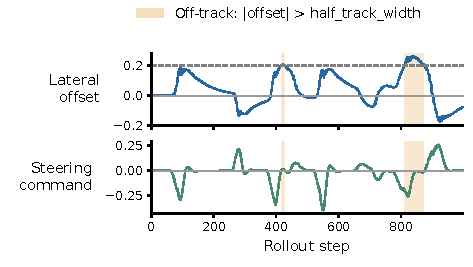
\includegraphics[width=\linewidth]{generated/recovery_edit_traces.pdf}
\end{minipage}\hfill
\begin{minipage}[t]{.485\linewidth}
\centering\textbf{\small (d) After: centering amplified when off-track}\\[3pt]
\resizebox{\linewidth}{!}{\begingroup
\let\ifincrementaledit\iftrue
% Shared grid and bounding box preserve alignment between panels (a) and (d).
\begin{tikzpicture}[x=1cm,y=1.3cm,>=Stealth,font=\fontsize{10}{11.5}\selectfont,
 var/.style={draw,line width=.65pt,inner sep=3pt,minimum height=.62cm,align=center},
 latent/.style={var,draw=blue!65!black,fill=blue!9},
 weight/.style={var,draw=orange!75!black,fill=orange!16},
 action/.style={var,draw=green!40!black,fill=green!12},
 op/.style={draw=black!65,dashed,rounded corners=3pt,inner sep=3pt,minimum height=.5cm,align=center},
 new/.style={line width=1pt},
 flow/.style={->,line width=.65pt},
 added/.style={->,draw=teal!65!black,line width=1pt}]
\path[use as bounding box] (-1.4,.45) rectangle (7.75,-5.65);
\node[latent,text width=2cm] (offset) at (1.2,0) {Lateral offset\\$x$};
\node[weight,text width=1.4cm] (weight) at (-.6,-1.35) {Centering\\weight};
\node[op,text width=1.35cm] (mul) at (1.2,-1.35) {multiply};
\node[latent,text width=2cm] (center) at (1.2,-2.55) {Centering\\contribution};
\node[latent,text width=2.2cm] (other) at (5.5,-3.65) {Other steering\\contributions};
\node[op,text width=1.35cm] (sum) at (5.5,-4.5) {add};
\node[action,text width=2cm] (steer) at (5.5,-5.35) {Steering\\command};
\draw[flow](offset.south)--(mul.north);
\draw[flow](weight.east)--(mul.west);
\draw[flow](mul.south)--(center.north);
\draw[flow](other.south)--(sum.north);
\draw[flow](sum.south)--(steer.north);
\ifincrementaledit
 \node[latent,new,text width=4cm] (off) at (5.5,0)
   {Off-track indicator\\$\max(|x|-$\\$\texttt{half\_track\_width},0)$};
 \node[weight,new,text width=1.5cm] (strength) at (3.2,-1.35)
   {Off-track\\strength\\$k\geq0$};
 \node[op,new,text width=2cm,draw=teal!65!black] (product) at (5.5,-1.35)
   {multiply, then $+1$};
 \node[latent,new,text width=2.2cm] (recovery) at (5.5,-2.55)
   {Recovery\\multiplier};
 \node[op,new,text width=1.35cm,draw=teal!65!black] (boost) at (1.2,-4.5)
   {multiply};
 \draw[added](offset.east)--(off.west);
 \draw[added](off.south)--(product.north);
 \draw[added](strength.east)--(product.west);
 \draw[added](product.south)--(recovery.north);
 \draw[added](recovery.west)--(3.25,-2.55)--(3.25,-3.6)--(1.2,-3.6)--(boost.north);
 \draw[flow](center.west)--(-.2,-2.55)--(-.2,-4.5)--(boost.west);
 \draw[added](boost.east)--(sum.west);
\else
 \draw[flow](center.west)--(-.2,-2.55)--(-.2,-4.5)--(sum.west);
\fi
\end{tikzpicture}

\endgroup
}
\end{minipage}
\caption{Example of off-track recovery structure refinement.
(a) The steering structure before refinement (other nodes ommitted);
(b) The desired behavior of re-centering, corresponding test, and the result;
(c) Recorded lateral offset and steering;
(d) The refined structure added a strong steering when the race car is off-track.
}
\label{fig:latent-traces}
\end{figure}


\subsection{Generating analysis code from the policy structure}
\label{sec:diagnostics}

By capturing semantics, the policy structure provides an interface for detailed inspection and localizing issues in each subgraph.
As when generating unit tests in software development, we instruct the LLM to reflect on expected behaviors and generate corresponding tests.
Given the task description and current structure $\llbracket \alpha^{(i)} \rrbracket$, the LLM proposes hypotheses and writes Python analysis functions $T^{(i)}_j$ to test each of the hypothesis.

Figure~\ref{fig:latent-traces}(b) illustrates one hypothesis: the policy should attempt to recenter after the car goes off-track.
The policy structure connects this hypothesis to a specific editable computation: the centering contribution generated from lateral offset (subgraph shown in Figure \ref{fig:latent-traces} (a)).
The test directly queries relevant variables (e.g., \texttt{offset}). We take advantage of the flexibility of Python syntax have no limit on what kind of tests it can generate.
The above example filters off-track time steps and measures the percentage of the policy exhibiting recovery behavior.

As these tests specify general desired behavior, they can be generated directly from the policy structure, independently of actual rollouts.
It shows a unique advantage: exposing semantic latents lets the LLM test specific questions, such as whether a steering contribution sufficiently influences off-track behavior, rather than inspecting only the aggregate action.
During each iteration the LLM generates multiple tests, each testing an individual behavior and subgraph of the policy.
Other generated analyses examine action saturation, reconstruction errors, and speed regulation (Appendix~\ref{app:diagnostic-prompts}).

\subsection{Collecting tabular trajectories from policy rollouts}
\label{sec:traces}

After training $\pi_{\langle \alpha^{(i)}, \Theta^{(i)} \rangle}$, we execute it and collect trajectories for analysis.
At each time step, the policy takes in the current state $s_t$ and populates all the latent values $z^{(i)}_{0,t}, z^{(i)}_{1,t}, \dots, z^{(i)}_{k,t}$ in its computation graph $\llbracket \alpha^{(i)} \rrbracket$.
Therefore, in addition to the output distribution $a_t$, it also returns all of the intermediate latent states, such as $\texttt{lateral\_offset}_t = 0.1$.
We organize observations, latents, parameters, and actions into a tabular trajectory,
\begin{equation}
    X^{(i)}[t,:]=[s_t,z^{(i)}_{0,t}, z^{(i)}_{1,t}, \dots, z^{(i)}_{k,t},\Theta^{(i)},a_t,s_{t+1}]
    \label{eq:trace}
\end{equation}
where each row records the current state, intermediate latents, weights, action output, and next state.

Figure~\ref{fig:latent-traces}(c) plots these two recorded columns over the full 1,000-step rollout.
The traces show the raw values supplied to the recovery behavior code analysis.
This shows the advantage of a semantic latent space: recorded trajectories contain not only states and actions but also the physical meaning of the intermediate computations that generate each action.

\subsection{Executing the analysis code and revising the policy structure}
\label{sec:revision}

We execute tests $T^{(i)}$ for desired behaviors on rollout $X^{(i)}$ through a Python interpreter and collect their outputs.
The tests can be applied to arbitrarily long rollouts or large rollout tables without exceeding the LLM's context length. Their results indicate whether the policy meets each criterion and, if not, which part of its structure is suboptimal.

In Figure~\ref{fig:latent-traces}(b), the test finds center-directed steering in only $14.9\%$ of off-track steps.
It identifies a state-dependent discrepancy: the executed policy rarely selects center-directed steering where the analysis expects recovery when the race car is off the track. This motivates a structural update making the steering more aggressive when the race car is off the track.

The LLM revises the structure using the task description, current structure, analysis code, and analysis outputs.
Edits can change dependencies, operations, latent variables, coefficient constraints, and initialization.
Figure~\ref{fig:latent-traces}(d) shows the recovery branch after the revision.
The revised program adds a pathway explicitly handling off-track behavior.
It computes an off-track indicator measuring excess lateral offset, scales it by a trainable nonnegative recovery strength, and adds one to form a multiplier.
% \begin{equation}
%     o_t=\max(|x_t|-h,0)\qquad
%     m_t=1+k o_t\qquad
%     c_t^{\mathrm{recovery}}=m_t w_x x_t\qquad k\geq0
%     \label{eq:recovery-edit}
% \end{equation}
% where $h=\texttt{half\_track\_width}$ and $w_x x_t$ is the original centering contribution.
% Within the track boundary, the multiplier is one; beyond it, the multiplier increases with excess offset when $k>0$.
The additional operations make recovery strength depend explicitly on the state while retaining the other steering contributions.
The program exposes the new indicator as \texttt{latent\_offtrack\_amount}, allowing subsequent data analysis code to inspect when this branch is active.

The illustrated change creates a \textbf{structural update}, rather than merely changing a fitted parameter.
Multiple analysis scripts may expose several issues in the structured policy during each update iteration, and the LLM is instructed to address all of them in that iteration.
The revised structure then repeats the cycle of training, expected-behavior test generation, rollout inspection, and revision.

\subsection{Reinforcement learning on the demonstration-aligned structure}
\label{sec:rl-method}

Reinforcement learning further optimizes parameters for reward, starting from the policy aligned through iterative refinement and demonstration fitting.
We hold the program fixed and use a critic-free, group-relative policy-gradient update adapted from GSPO~\citep{zheng2025group}.
Trajectories begin from a shared initial condition; time-aligned reward-to-go estimates supply relative advantages, and action windows supply the likelihood ratios.
We form each ratio from the product of action likelihoods within its window (Appendix~\ref{app:rl}).
This stage follows structural refinement; imitation learning remains the parameter-fitting step inside the loop.
The deployed controller executes the final fitted program without LLM calls.

\section{Experiments and analysis}
\label{sec:experiments}
% Target: 2.5 pages. Reuse IJCAI26 evidence only; KIM results are not new results.
% Source mapping: content_mapping.md, Sections 5.1--5.5.

\subsection{Tasks, baselines, and evaluation protocol}
\label{sec:setup}
\begin{itemize}
    \item Describe low-dimensional Car Racing and Door Opening, one
    demonstration per task, demonstration provenance, and the ten reported
    unseen evaluation settings. Verify reward definitions, horizons, and
    separation between refinement rollouts and final evaluation settings.
    \item Introduce zero-shot structured policy as the primary refinement
    comparison; MLP and MLES provide context. Specify training stages and the
    different supervision/resources available to each baseline.
    \item State the LLM configuration, refinement/training budgets, metrics,
    and what each uncertainty estimate aggregates. Recover independent-run
    counts; do not equate evaluation settings with independent training runs.
\end{itemize}

\subsection{Does iterative refinement improve the initial policy?}
\label{sec:refinement-results}
\begin{itemize}
    \item Lead with the existing zero-shot versus refined Car Racing imitation
    results and the reported performance across iterations. Distinguish changes
    in fitted behavior from the untested claim of recovering the expert's strategy.
    \item Include Door Opening's reach-and-pull progression and distance metric
    as the second task. Report limited progress in intermediate iterations;
    avoid claiming that every revision produces an improvement.
    \item Plan a compact performance table and refinement-history figure using
    existing data/figures where recoverable. Keep resource columns separate
    from reward, and preserve the uncertainty definitions.
\end{itemize}

\subsection{How does the feedback affect refinement?}
\label{sec:feedback-results}
\begin{itemize}
    \item Compare generated-analysis results, subsampled trajectory tables,
    and no-feedback revision using the existing Car Racing comparison. Explain
    the table-subsampling and matched-budget details that must be recovered.
    \item Reuse the input/output token table and discuss both counts, including
    the larger output budget for analysis generation. Do not turn token counts
    into unmeasured latency, monetary cost, or total-compute savings.
    \item State the ablation's scope: it evaluates feedback procedures, not an
    isolated effect of semantic names or latent logging. No reward-only feedback
    result is present in the source manuscript.
\end{itemize}

\subsection{What changes across refinement iterations?}
\label{sec:edit-analysis}
\begin{itemize}
    \item Extend the matched method example into a compact iteration record:
    observed issue, diagnostic evidence, edit type, and subsequent behavior.
    Separate documented explanations from conjectured mechanisms. Use the
    method's running example to establish the workflow, and this subsection
    for evidence across revisions rather than retelling the same example.
    \item Reuse the existing Door Opening narrative, diagnostic categories,
    and manually coded strategy-coverage table selectively. Explain the manual
    coding procedure; move full coverage tables to the appendix.
    \item Include ineffective revisions and diagnostic blind spots where
    documented. Recover per-iteration programs/logs to distinguish additions,
    operation/constraint changes, and initialization changes.
\end{itemize}

\subsection{Does refinement help subsequent reinforcement learning?}
\label{sec:rl-results}
\begin{itemize}
    \item Present the reported refined versus zero-shot policy outcomes at the
    stated RL budgets as a downstream benefit. Briefly explain when RL begins;
    keep its detailed derivation in Appendix~\ref{app:rl}.
    \item Separate refinement resets, RL resets, and LLM calls. Audit the old
    abstract's compute percentage against the table; report environment resets
    as such, without claiming measured total-compute savings or statistical
    equivalence from similar mean returns.
\end{itemize}

\section{Discussion and conclusion}
\label{sec:conclusion}
% Target: 0.5 page. Source mapping: content_mapping.md, Sections 6.1--6.2.

\subsection{Scope and limitations}
\label{sec:limitations}
\begin{itemize}
    \item Discuss reliance on initial LLM knowledge, authored feature/task
    descriptions, and generated tests that can miss failures or encode incorrect
    expectations. The study does not establish recovery from arbitrary initial
    misalignment or verified semantic correctness.
    \item Bound the evidence to two low-dimensional simulated tasks. State
    limits of run variability and attribution where unresolved; distinguish
    behavioral improvement from proof of causal structure or the expert's
    internal decision process.
\end{itemize}

\subsection{Takeaway}
\label{sec:takeaway}
\begin{itemize}
    \item Close with the supported role of semantic execution analysis in
    iterative structural refinement and improved policy learning in the tested
    settings. Keep the representation attributed to prior work and the
    refinement process as the paper's contribution.
\end{itemize}


% The style hides this environment during anonymous review.
\begin{ack}
% Add acknowledgments and disclosures for the accepted version only.
\end{ack}

\bibliographystyle{plainnat}
% Enable when research citations are added; this outline has no citations yet.
% \bibliography{references}

% The NEmo call does not currently specify whether a checklist is required.
% The official checklist is retained; enable and complete if requested.
% \clearpage
% \input{vendor/neurips2026/checklist}

\clearpage
\appendix
% Outline only. References/appendices are outside the eight-page main-text budget.
% Source mapping: content_mapping.md, Appendices A--E.

\section{Policy-generation prompts and interfaces}
\label{app:generation}

\subsection{Shared generation specification}
\label{app:specification}
\begin{itemize}
    \item Reuse the IJCAI26 policy-generation specification: semantic variables,
    differentiable computation, parameter initialization, action-distribution
    outputs, and the logging dictionary. Preserve prompts used in experiments;
    distinguish historical prompt text from any corrected explanatory text.
\end{itemize}

\subsection{Environment descriptions and observation schemas}
\label{app:environment}
\begin{itemize}
    \item Reuse the Car Racing and Door Opening environment prompts, feature
    shapes, sign conventions, action spaces, and task information. Verify these
    against the actual experiment interface before drafting.
\end{itemize}

\section{Diagnostic and revision prompts}
\label{app:prompts}

\subsection{Hypothesis generation and analysis execution}
\label{app:diagnostic-prompts}
\begin{itemize}
    \item Include the shared diagnostic system prompt, policy/schema input
    template, result format, and execution details. Show full scripts for the
    main example and document error handling from actual implementation records.
\end{itemize}

\subsection{Revision, additional tests, and termination}
\label{app:revision-prompts}
\begin{itemize}
    \item Reuse all three response branches from the refinement prompt. Add
    the actual orchestration, budget, stopping, and any selection rules from
    experiment records; identify behavior not documented by the old paper.
\end{itemize}

\section{Training and evaluation details}
\label{app:training}

\subsection{Imitation learning and refinement configuration}
\label{app:il}
\begin{itemize}
    \item Provide optimizer settings, initialization/transfer behavior, training
    stopping criteria, LLM configuration, rollout seeds, evaluation separation,
    independent-run counts, and uncertainty calculations from saved records.
\end{itemize}

\subsection{Post-refinement reinforcement learning}
\label{app:rl}
\begin{itemize}
    \item Adapt the IJCAI26 RL subsection after checking objective, sequence
    grouping, indexing, and implementation consistency. State the assumption
    behind grouping states at corresponding times across sampled trajectories.
    Document RL hyperparameters and exact reset accounting.
\end{itemize}

\section{Complete refinement records}
\label{app:records}

\subsection{Car Racing programs, diagnostics, and rollouts}
\label{app:car-record}
\begin{itemize}
    \item Recover the before/after programs, demonstration-fitting details,
    relevant log rows, full diagnostic outputs, and post-refit evaluations for
    the main example. Record provenance and iteration identifiers.
\end{itemize}

\subsection{Door Opening progression}
\label{app:door-record}
\begin{itemize}
    \item Expand the existing iteration images and narrative with matched
    programs/diagnostics where available. Preserve ineffective intermediate
    revisions and distinguish measured distance from qualitative task success.
\end{itemize}

\section{Extended feedback and semantic analyses}
\label{app:extended}

\subsection{Diagnostic and strategy coverage}
\label{app:coverage}
\begin{itemize}
    \item Reuse the detailed diagnostic-coverage and semantic-strategy tables.
    Explain manual categories, coding criteria, and limits of coverage counts
    as measures of semantic correctness or diagnostic usefulness.
\end{itemize}

\subsection{Feedback budgets and supplementary results}
\label{app:budgets}
\begin{itemize}
    \item Document raw-table subsampling, feedback comparability, token
    aggregation, refinement histories, and supplementary baseline/RL rows from
    existing records. Do not populate missing measurements with inferred data.
\end{itemize}

\end{document}
